\scanpage{34}
\mspage{1}
Systèmes spéciaux de cinq points sur une sphère complexe (plus gén.\textsuperscript{t} sur une \deleted{\unsure{courbe}} droite projective sur un corps alg clos \(k\) \unsure{de car. \(0\)})

Ce sont les systèmes \((\Sigma,I)\) où \(K\subset\Sigma\), \(\operatorname{card}K=5\), et tels qu’il existe un autom. non trivial de \((\Sigma,K)\) --- i.e. le groupe \inserted{\(G\)} des automorphismes de \((\Sigma,K)\) n’est pas réduit à \(1\). On fait la classification suivant la structure de ce groupe.

Soit \(g\in G\) d’ordre maximal. On peut identifier \(g\) à une permutation de \(I\), et la discussion se fait suivant la structure de celle-ci. Notons que \deleted{l’ordre de \(g\ne1\) est} tout autom. d’ordre fini de \(\Sigma\) \deleted{\(g\) d’ordre \(5\)} a exactement deux pts fixes, et que \deleted{\unsure{il est}} \inserted{si l’ordre est \(\nu\)}, \(\mathbb Z/\nu\mathbb Z\) opère librement sur \(\Sigma\setminus\Sigma^g\). Cela montre que
\[
K=K^g\amalg\text{orbites d’ordre }\nu,\quad\text{donc }2\leq\nu\leq5.
\]
\margin{l’opération est celle de \(\mu_\nu\) sur \(\mathbb G_m\).}

\textcircled{1} \(\nu=5\), alors \(K\) est une orbite --- OPS qui est l’orbite \(\mu_5(k)\) de \(\mu_5\) opérant sur \(\mathbb P^1_k\). Le groupe total des autom. est \(\mathbb D_5\). À isom. près, il y a un seul tel cas.

\margin{Structure pentagonale sur \(I\) (``pentagone'')}
\figure{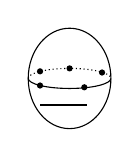
\begin{tikzpicture}[scale=.75]
\draw (0,0) ellipse(.7 and .85);
\draw (-.7,0) arc[start angle=180,end angle=360,x radius=.7,y radius=.17];
\draw[densely dotted] (-.7,0) arc[start angle=180,end angle=0,x radius=.7,y radius=.17];
\foreach \x/\y in {-.5/-.12,.25/-.15,.55/.1,-.5/.12,0/.17}{\fill(\x,\y)circle(1.5pt);}
\draw(-.5,-.45)--(.3,-.45);
\end{tikzpicture}}

\textcircled{2} \(\nu=4\) alors \deleted{\(\unsure{K^g}=\operatorname{card}I^g=1\)} \inserted{\(K^g=\{P\}\)}, et \(I\setminus\{P\}\) est une orbite. OPS que c’est \(\mu_4\), sur lequel \(\mu_4\) opère, et \(P\) est un pôle : \(\infty\). Le groupe total des autom. est \(\mathbb Z/4\mathbb Z\simeq\mu_4(k)\).

La catégorie de ces configurations est équivalente à celle des carrés orientés.

\margin{``pyramide carrée''}
\figure{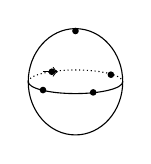
\begin{tikzpicture}[scale=.75]
\draw(0,0)ellipse(.8 and .9);
\draw(-.8,0)arc[start angle=180,end angle=360,x radius=.8,y radius=.2];
\draw[densely dotted](-.8,0)arc[start angle=180,end angle=0,x radius=.8,y radius=.2];
\foreach \x/\y in {0/.86,-.55/-.14,.3/-.18,.6/.12,-.4/.17}{\fill(\x,\y)circle(1.6pt);}
\draw[->](-.55,.17)--(-.3,.17);
\end{tikzpicture}}

\textcircled{3} \(\nu=3\), Alors \deleted{\(\unsure{K}\)} \(\operatorname{card}K^g=2\), \inserted{donc \(K^g=\Sigma^g\)}, et \(I\setminus K^g\) \inserted{\(=J\)} une orbite,
\deleted{Le groupe total des}
qu’on peut \unsure{supposer} \(\mu_3\). La catégorie de ces configurations est équivalente à celle des triangles combinatoires i.e. celle \(\mathrm{Ens}(3)\) des ens \(J\) de card \(3\).

À \(J\) on associe \(\Sigma_J\deleted{\unsure{\Sigma}}\) avec \(J\cup P_J\) (\(P_J\subset\Sigma_J\) ens des deux pôles de \(\Sigma_J\) en corr. \(1\)-\(1\) avec l’ens \(\omega(J)\) des or. de \(J\), si \(k=\mathbb C\)). Groupe des autom. est \(\mathbb D_3\).

\margin{\unsure{Partition} \(2\) et \(3\) (par ordre de \unsure{cardinaux|valeurs} ou \unsure{symétries})}
\margin{``bitétraèdre''}
\figure{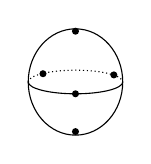
\begin{tikzpicture}[scale=.75]
\draw(0,0)ellipse(.8 and .9);
\draw(-.8,0)arc[start angle=180,end angle=360,x radius=.8,y radius=.2];
\draw[densely dotted](-.8,0)arc[start angle=180,end angle=0,x radius=.8,y radius=.2];
\foreach \x/\y in {0/.86,0/-.84,0/-.2,-.55/.14,.65/.12}{\fill(\x,\y)circle(1.7pt);}
\end{tikzpicture}}
\mspage{33}
